\documentclass{standalone}
\usepackage{tikz}
\usetikzlibrary{patterns, positioning}

\begin{document}
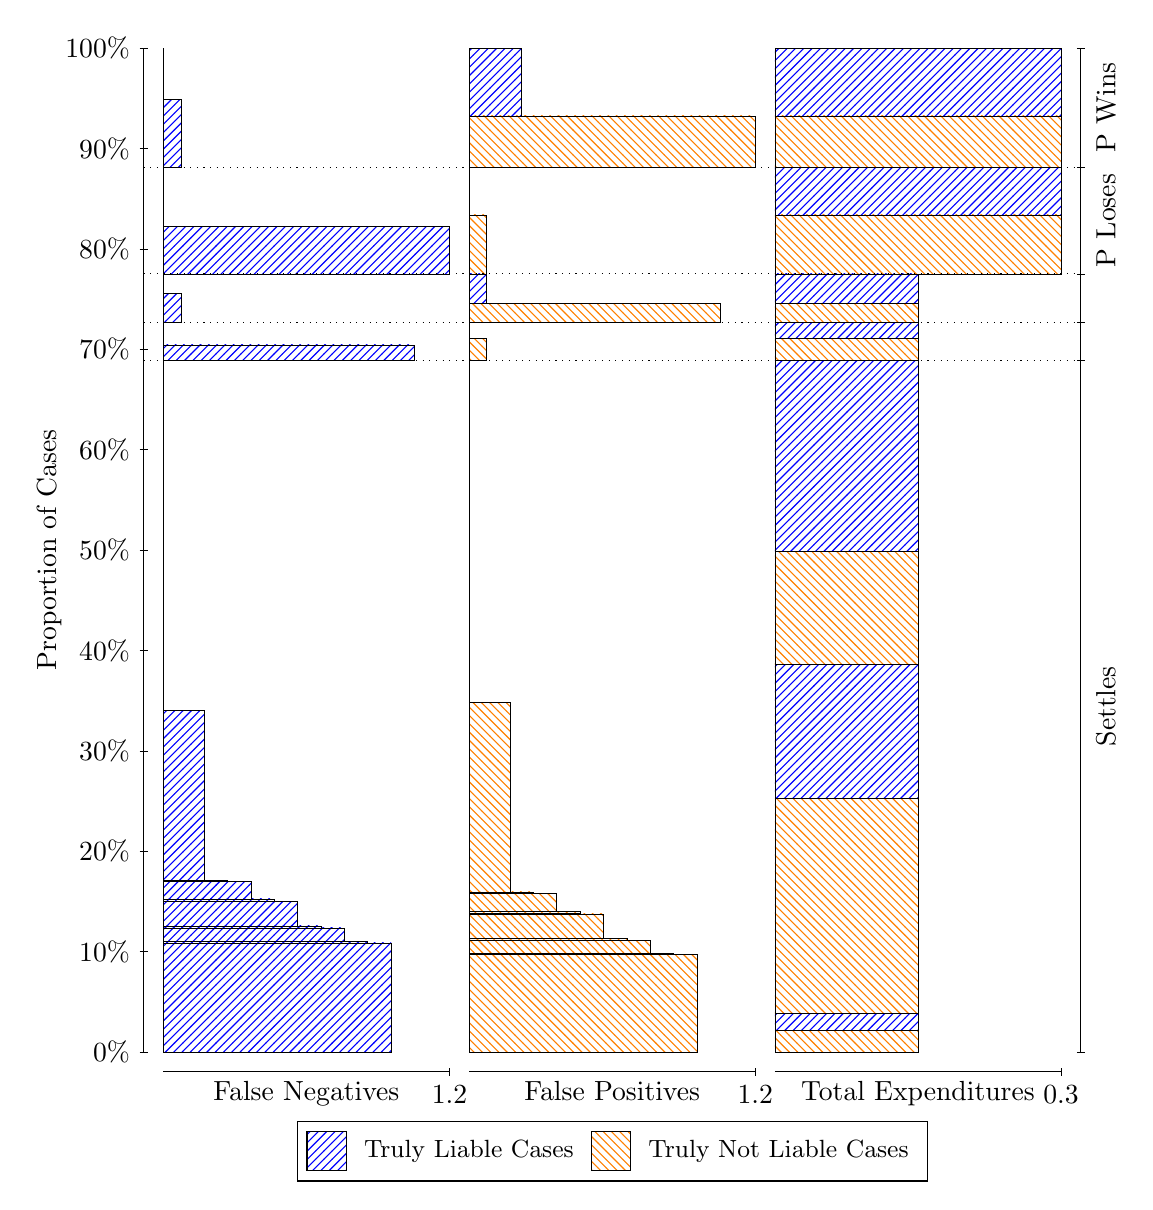
\begin{tikzpicture}
\draw[black, very thin] (1.5,1.75) -- (1.5,14.5);
\node[rotate=90, anchor=center] at (0.3, 8.125) {Proportion of Cases};
\draw[black, very thin] (1.45,1.75) -- (1.55,1.75);
\node[anchor=east] at (1.45, 1.75) {0\%};
\draw[black, very thin] (1.45,3.025) -- (1.55,3.025);
\node[anchor=east] at (1.45, 3.025) {10\%};
\draw[black, very thin] (1.45,4.3) -- (1.55,4.3);
\node[anchor=east] at (1.45, 4.3) {20\%};
\draw[black, very thin] (1.45,5.575) -- (1.55,5.575);
\node[anchor=east] at (1.45, 5.575) {30\%};
\draw[black, very thin] (1.45,6.85) -- (1.55,6.85);
\node[anchor=east] at (1.45, 6.85) {40\%};
\draw[black, very thin] (1.45,8.125) -- (1.55,8.125);
\node[anchor=east] at (1.45, 8.125) {50\%};
\draw[black, very thin] (1.45,9.4) -- (1.55,9.4);
\node[anchor=east] at (1.45, 9.4) {60\%};
\draw[black, very thin] (1.45,10.675) -- (1.55,10.675);
\node[anchor=east] at (1.45, 10.675) {70\%};
\draw[black, very thin] (1.45,11.95) -- (1.55,11.95);
\node[anchor=east] at (1.45, 11.95) {80\%};
\draw[black, very thin] (1.45,13.225) -- (1.55,13.225);
\node[anchor=east] at (1.45, 13.225) {90\%};
\draw[black, very thin] (1.45,14.5) -- (1.55,14.5);
\node[anchor=east] at (1.45, 14.5) {100\%};

\draw[black, very thin] (13.4,1.75) -- (13.4,14.5);
\draw[black, very thin] (13.35,1.75) -- (13.45,1.75);
\node[anchor=west] at (13.35, 1.75) {};
\draw[black, very thin] (13.35,10.533) -- (13.45,10.533);
\node[anchor=west] at (13.35, 10.533) {};
\draw[black, very thin] (13.35,11.013) -- (13.45,11.013);
\node[anchor=west] at (13.35, 11.013) {};
\draw[black, very thin] (13.35,11.631) -- (13.45,11.631);
\node[anchor=west] at (13.35, 11.631) {};
\draw[black, very thin] (13.35,12.985) -- (13.45,12.985);
\node[anchor=west] at (13.35, 12.985) {};
\draw[black, very thin] (13.35,14.5) -- (13.45,14.5);
\node[anchor=west] at (13.35, 14.5) {};

\draw[black, very thin, pattern color=blue, pattern=north east lines] (1.75,1.75) rectangle (4.6418,3.1362);
\draw[black, very thin, pattern color=blue, pattern=north east lines] (1.75,3.1362) rectangle (4.3452,3.1531);
\draw[black, very thin, pattern color=blue, pattern=north east lines] (1.75,3.1531) rectangle (4.0486,3.3272);
\draw[black, very thin, pattern color=blue, pattern=north east lines] (1.75,3.3272) rectangle (3.752,3.3506);
\draw[black, very thin, pattern color=blue, pattern=north east lines] (1.75,3.3506) rectangle (3.4554,3.6672);
\draw[black, very thin, pattern color=blue, pattern=north east lines] (1.75,3.6672) rectangle (3.1588,3.6934);
\draw[black, very thin, pattern color=blue, pattern=north east lines] (1.75,3.6934) rectangle (2.8622,3.9123);
\draw[black, very thin, pattern color=blue, pattern=north east lines] (1.75,3.9123) rectangle (2.5656,3.9263);
\draw[black, very thin, pattern color=blue, pattern=north east lines] (1.75,3.9263) rectangle (2.269,6.0888);
\draw[black, very thin, pattern color=orange, pattern=north west lines] (1.75,6.0888) rectangle (1.75,10.533);
\draw[black, very thin, pattern color=blue, pattern=north east lines] (1.75,10.533) rectangle (4.9384,10.731);
\draw[black, very thin, pattern color=orange, pattern=north west lines] (1.75,10.731) rectangle (1.75,11.013);
\draw[black, very thin, pattern color=blue, pattern=north east lines] (1.75,11.013) rectangle (1.9724,11.386);
\draw[black, very thin, pattern color=orange, pattern=north west lines] (1.75,11.386) rectangle (1.75,11.631);
\draw[black, very thin, pattern color=blue, pattern=north east lines] (1.75,11.631) rectangle (5.3833,12.234);
\draw[black, very thin, pattern color=orange, pattern=north west lines] (1.75,12.234) rectangle (1.75,12.985);
\draw[black, very thin, pattern color=blue, pattern=north east lines] (1.75,12.985) rectangle (1.9724,13.847);
\draw[black, very thin, pattern color=orange, pattern=north west lines] (1.75,13.847) rectangle (1.75,14.5);
\draw[black, very thin, pattern color=orange, pattern=north west lines] (5.6333,1.75) rectangle (8.5252,2.9919);
\draw[black, very thin, pattern color=orange, pattern=north west lines] (5.6333,2.9919) rectangle (8.2286,3.0032);
\draw[black, very thin, pattern color=orange, pattern=north west lines] (5.6333,3.0032) rectangle (7.932,3.1666);
\draw[black, very thin, pattern color=orange, pattern=north west lines] (5.6333,3.1666) rectangle (7.6354,3.1878);
\draw[black, very thin, pattern color=orange, pattern=north west lines] (5.6333,3.1878) rectangle (7.3388,3.5046);
\draw[black, very thin, pattern color=orange, pattern=north west lines] (5.6333,3.5046) rectangle (7.0422,3.5115);
\draw[black, very thin, pattern color=orange, pattern=north west lines] (5.6333,3.5115) rectangle (7.0422,3.5311);
\draw[black, very thin, pattern color=orange, pattern=north west lines] (5.6333,3.5311) rectangle (6.7456,3.763);
\draw[black, very thin, pattern color=orange, pattern=north west lines] (5.6333,3.763) rectangle (6.449,3.7822);
\draw[black, very thin, pattern color=orange, pattern=north west lines] (5.6333,3.7822) rectangle (6.1524,6.1938);
\draw[black, very thin, pattern color=blue, pattern=north east lines] (5.6333,6.1938) rectangle (5.6333,10.533);
\draw[black, very thin, pattern color=orange, pattern=north west lines] (5.6333,10.533) rectangle (5.8558,10.814);
\draw[black, very thin, pattern color=blue, pattern=north east lines] (5.6333,10.814) rectangle (5.6333,11.013);
\draw[black, very thin, pattern color=orange, pattern=north west lines] (5.6333,11.013) rectangle (8.8218,11.258);
\draw[black, very thin, pattern color=blue, pattern=north east lines] (5.6333,11.258) rectangle (5.8558,11.631);
\draw[black, very thin, pattern color=orange, pattern=north west lines] (5.6333,11.631) rectangle (5.8558,12.382);
\draw[black, very thin, pattern color=blue, pattern=north east lines] (5.6333,12.382) rectangle (5.6333,12.985);
\draw[black, very thin, pattern color=orange, pattern=north west lines] (5.6333,12.985) rectangle (9.2667,13.638);
\draw[black, very thin, pattern color=blue, pattern=north east lines] (5.6333,13.638) rectangle (6.3007,14.5);
\draw[black, very thin, pattern color=orange, pattern=north west lines] (9.5167,1.75) rectangle (11.333,2.0276);
\draw[black, very thin, pattern color=blue, pattern=north east lines] (9.5167,2.0276) rectangle (11.333,2.242);
\draw[black, very thin, pattern color=orange, pattern=north west lines] (9.5167,2.242) rectangle (11.333,4.9704);
\draw[black, very thin, pattern color=blue, pattern=north east lines] (9.5167,4.9704) rectangle (11.333,6.6731);
\draw[black, very thin, pattern color=orange, pattern=north west lines] (9.5167,6.6731) rectangle (11.333,8.1109);
\draw[black, very thin, pattern color=blue, pattern=north east lines] (9.5167,8.1109) rectangle (11.333,10.533);
\draw[black, very thin, pattern color=orange, pattern=north west lines] (9.5167,10.533) rectangle (11.333,10.814);
\draw[black, very thin, pattern color=blue, pattern=north east lines] (9.5167,10.814) rectangle (11.333,11.013);
\draw[black, very thin, pattern color=orange, pattern=north west lines] (9.5167,11.013) rectangle (11.333,11.258);
\draw[black, very thin, pattern color=blue, pattern=north east lines] (9.5167,11.258) rectangle (11.333,11.631);
\draw[black, very thin, pattern color=orange, pattern=north west lines] (9.5167,11.631) rectangle (13.15,12.382);
\draw[black, very thin, pattern color=blue, pattern=north east lines] (9.5167,12.382) rectangle (13.15,12.985);
\draw[black, very thin, pattern color=orange, pattern=north west lines] (9.5167,12.985) rectangle (13.15,13.638);
\draw[black, very thin, pattern color=blue, pattern=north east lines] (9.5167,13.638) rectangle (13.15,14.5);
\draw[black, dotted] (1.5,10.533) -- (13.4,10.533);
\draw[black, dotted] (1.5,11.013) -- (13.4,11.013);
\draw[black, dotted] (1.5,11.631) -- (13.4,11.631);
\draw[black, dotted] (1.5,12.985) -- (13.4,12.985);
\draw[black, very thin] (1.75,1.5) -- (5.3833,1.5);
\node[anchor=north] at (3.5667, 1.5) {False Negatives};
\draw[black, very thin] (5.3833,1.45) -- (5.3833,1.55);
\node[anchor=north] at (5.3833, 1.45) {1.2};

\draw[black, very thin] (5.6333,1.5) -- (9.2667,1.5);
\node[anchor=north] at (7.45, 1.5) {False Positives};
\draw[black, very thin] (9.2667,1.45) -- (9.2667,1.55);
\node[anchor=north] at (9.2667, 1.45) {1.2};

\draw[black, very thin] (9.5167,1.5) -- (13.15,1.5);
\node[anchor=north] at (11.333, 1.5) {Total Expenditures};
\draw[black, very thin] (13.15,1.45) -- (13.15,1.55);
\node[anchor=north] at (13.15, 1.45) {0.3};

\node[black, centered, rotate=90] at (13.72, 6.1413) {Settles};


\node[black, centered, rotate=90] at (13.72, 12.308) {P Loses};
\node[black, centered, rotate=90] at (13.72, 13.743) {P Wins};

\draw (7.449999999999999,1.5) node[draw=none] (baseCoordinate) {};
\begin{scope}[align=center]
        \matrix[scale=0.5, draw=black, below=0.5cm of baseCoordinate, nodes={draw}, column sep=0.1cm]{
            \node[rectangle, draw, minimum width=0.5cm, minimum height=0.5cm, pattern=north east lines, pattern color=blue] {}; &
            \node[draw=none, font=\small] (B) {Truly Liable Cases}; &
            \node[rectangle, draw, minimum width=0.5cm, minimum height=0.5cm, pattern=north west lines, pattern color=orange] {}; &
            \node[draw=none, font=\small] (B) {Truly Not Liable Cases}; \\
            };
\end{scope}

\end{tikzpicture}
\end{document}